\section{假设检验}

假设检验是一种统计推断方法, 用于判断关于总体参数的某种假设是否成立. 在假设检验中, 我们通常会提出一个关于总体参数的假设, 然后利用样本数据来判断这个假设是否成立.

\subsection{假设检验的基本思想}

\begin{example}
    某厂生产一种袋装白糖, 每袋白糖的净重是一个随机变量, 服从正态分布 $ N\left(\mu, \sigma^{2}\right)$, \label{baitjq}
    机器正常工作时, 均值是 $0.5$ (单位: $ \mathrm{kg}$), 标准差是 $ 0.01 \mathrm{~kg}$, 某天随机地抽取 $5$ 袋白糖, 称得净重为
    $$\begin{array}{lllll}
            0.54 & 0.58 & 0.47 & 0.49 & 0.52
        \end{array}$$
    问当日机器是否正常工作?
\end{example}
\begin{solution}
    由题意知, 方差 $ \sigma^{2} $ 已知, $\mu $ 未知, 要判断机器是否正常工作, 就是要判断该日生产的白糖净重的均值是否为 $ 0.5 \mathrm{~kg} $,
    即检验假设“$\mu=0.5$”是否正确. 因此, 提出两个相互对立的假设:\\
    原假设 $ H_{0}: \mu=\mu_{0}=0.5 $, 备择假设 $ H_{1}: \mu \neq 0.5 .$\\
    如果假设 $ H_{0}: \mu=\mu_{0}=0.5 $ 为真, 那么机器正常工作; 如果假设 $ H_{1}: \mu \neq 0.5 $ 为真, 则机器工作不正常.\\
    在假设 $ H_{0}: \mu=\mu_{0}=0.5 $ 条件下, 统计量 $\displaystyle Z=\frac{\bar{X}-\mu_{0}}{\sigma / \sqrt{n}} \sim N(0,1) $,
    由标准正态分布的分位点的定义 (见图 \ref{alphafweidian}), 知 $ P_{\mu_{0}}\left\{\left|\frac{\bar{X}-\mu_{0}}{\sigma / \sqrt{n}}\right| \geqslant z_{\alpha / 2}\right\}=\alpha $,
    若给定 $ \alpha=0.05$, 查表知 $ z_{0.025}=1.96$, 代人样本数据: $ n=5, \bar{x}=0.52 $,
    则 $$\displaystyle z=\frac{\bar{x}-\mu_{0}}{\sigma / \sqrt{n}}=\frac{0.52-0.5}{0.01 / \sqrt{5}}=4.47>1.96 .$$

    这说明小概率事件发生了, 所以应该拒绝假设 $ H_{0}: \mu=\mu_{0}=0.5 $, 接受备择假设 $ H_{1}: \mu \neq 0.5 $, 即机器工作不正常.
\end{solution}

\begin{definition}[接收域和拒绝域]
    \index{接收域和拒绝域}
    上述例题中, 若 $ z $ 取值在区间 $ (-1.96,1.96) $ 范围内, 则接受假设 $ H_{0} $, 即 $ |z|<z_{\alpha / 2} $ 称为\textit{接受域},
    而 $ |z| \geqslant z_{\alpha / 2} $ 称为\textit{拒绝域}, $z_{\alpha / 2} $ 称为\textit{临界值}, $\displaystyle Z=\frac{\bar{X}-\mu_{0}}{\sigma / \sqrt{n}} $ 称为\textit{检验统计量}.
\end{definition}

在根据样本作推断时, 由于样本的随机性, 难免会做出错误的决定.

\begin{definition}[第一类错误]
    \index{第一类错误}当原假设 $ H_{0} $ 为真时, 而做出拒绝 $ H_{0} $ 的判断, 称为犯\textit{第一类错误} (\textit{拒真错误})
    \label{category_1Errors}
\end{definition}

\begin{definition}[第二类错误]
    \index{第二类错误}当原假设 $ H_{0} $ 不真时, 而作出接受 $ H_{0} $ 的判断, 称为犯\textit{第二类错误} (\textit{取伪错误}).
\end{definition}

\begin{definition}[显著性水平]
    \index{显著性水平}在实际应用中, 控制犯第一类错误的概率, 使其不大于一个较小的正数 $ \alpha~(0<\alpha<1)$, 称 $ \alpha $ 为检验的\textit{显著性水平}.
\end{definition}

\begin{definition}[双边备择假设与双边假设检验]
    \index{双边备择假设与双边假设检验}
    形如 $ H_{1}: \mu \neq \mu_{0} $ 的假设, 表示 $ \mu $ 可能大于 $ \mu_{0} $, 也可能小于 $ \mu_{0}$, 称为\textit{双边备择假设};
    形如 $ H_{0}: \mu=\mu_{0} $ 的假设, 称为\textit{双边假设检验}.
\end{definition}

在实际中, 有时只关心均值是否减小. 例如某机器的生产效率问题, 此时我们应该关注的是生产时间, 时间越短越好.
对于采用新工艺来提高生产效率, 生产时间是否显著缩短的问题, 需要考虑如下假设检验:
原假设 $ H_{0}: \mu \geqslant \mu_{0}$, 备择假设 $ H_{1}: \mu<\mu_{0} .$

\begin{definition}[单边检验]
    \index{单边检验}
    形如 $ H_{0}: \mu \geqslant \mu_{0} $ 的假设称为\textit{左边检验}, 类似的形如 $ H_{0}: \mu \leqslant \mu_{0} $ 的假设称为\textit{右边检验}.
    左边检验和右边检验统称为\textit{单边检验}.
\end{definition}

假设检验的解题步骤:
\begin{enumerate}[label=(\arabic{*})]
    \item 确定原假设 $H_0$ 与备择假设 $H_1$;
    \item 选择合适的检验统计量, 在原假设成立的条件下求其发布;
    \item 根据显著性水平 $\alpha$, 再原假设成立的条件下确定临界值和拒绝域;
    \item 判断是否落入拒绝域, 落入拒绝域则拒绝 $H_0$, 否则拒绝 $H_1$.
\end{enumerate}

\begin{example}
    在假设检验时, 对于 $H_0:u=u_0,H_1:u\neq u_0$, 称 $(\quad)$ 为反第一类错误
    \begin{tasks}(2)
        \task $H_1$ 真, 接受 $H_1$.
        \task $H_1$ 不真, 接受 $H_1$.
        \task $H_1$ 真, 拒绝 $H_1$.
        \task $H_1$ 不真, 拒绝 $H_1$.
    \end{tasks}
\end{example}
\begin{solution}
    由定义 \ref{category_1Errors} 可知, 选 B.
\end{solution}

\subsection{单个正态总体的假设检验}

\subsubsection{\texorpdfstring{$\sigma^2$}. 已知, 关于 \texorpdfstring{$\mu$}. 的检验 (\texorpdfstring{$Z$}. 检验)}

设总体 $ X \sim N\left(\mu, \sigma^{2}\right)$, 其中 $ \sigma^{2} $ 已知, 要检验假设:
\begin{enumerate}[label=(\arabic{*})]
    \item 双边检验. $ H_{0}: \mu=\mu_{0} $, 备择假设 $ H_{1}: \mu \neq \mu_{0} $,
          由例题 \ref{baitjq} 知, 选取检验统计量为 $\displaystyle Z=\frac{\bar{X}-\mu_{0}}{\sigma / \sqrt{n}}$, 拒绝域为 $ |z| \geqslant z_{\alpha / 2} .$
    \item 右边检验. $ H_{0}: \mu \leqslant \mu_{0}, H_{1}: \mu>\mu_{0} $,
          选择统计量 $\displaystyle Z=\frac{\bar{X}-\mu_{0}}{\sigma / \sqrt{n}} \sim N(0,1) $, 根据标准正态分布分位点的定义 (见图 \ref{biaozfweidian}(a)) 可知 $\displaystyle P_{\mu_{0}}\left\{\frac{\bar{X}-\mu_{0}}{\sigma / \sqrt{n}} \geqslant z_{\alpha}\right\}=\alpha $, 则拒绝域为 $ z \geqslant z_{\alpha} .$
    \item 左边检验. $ H_{0}: \mu \geqslant \mu_{0}, H_{1}: \mu<\mu_{0} $,
          选取统计量 $\displaystyle  Z=\frac{\bar{X}-\mu_{0}}{\sigma / \sqrt{n}} \sim N(0,1)$, 由标准正态分布分位点的定义 (见图 \ref{biaozfweidian}(b)) 可知 $\displaystyle P_{\mu_{0}}\left\{\frac{\bar{X}-\mu_{0}}{\sigma / \sqrt{n}} \leqslant-z_{\alpha}\right\}=\alpha$, 则拒绝域为 $ z \leqslant-z_{\alpha} .$
\end{enumerate}

\begin{figure}[H]
    \centering
    \subfigure[]{
        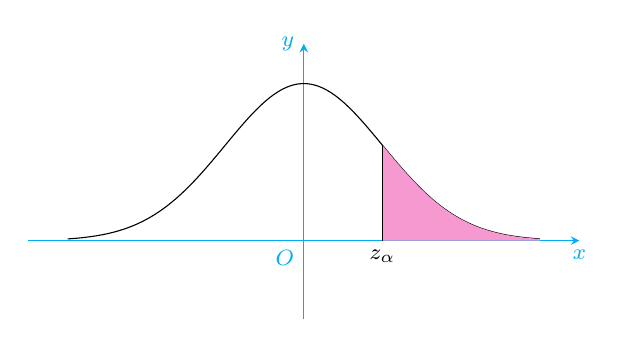
\begin{tikzpicture}[->,samples=100,>=stealth,font=\footnotesize,yscale=5]
            \def\xmin{-3.5}
            \def\xmax{3.5}
            \def\ymin{-.2}
            \def\ymax{.5}
            \def\a{0.398942}
            \draw[->,cyan](\xmin,0)--(0,0)node[below left]{$O$}--(\xmax,0)node[below]{$x$};
            \draw[->,cyan](0,\ymin)--(0,\ymax)node[left]{$y$};

            \draw[scale=1,domain=-3:3,smooth,variable=\x,black,-] plot ({\x},{\a*exp(-\x*\x/2)});

            \fill[color=magenta!40] (1,0) -- plot[domain=1:3,smooth,variable=\x] ({\x},{\a*exp(-\x*\x/2)}) -- (3,0) --cycle;
            \node[below] at (1,0) {$z_{\alpha}$};
            \draw[-] (1,0)--plot[domain=1:1,smooth,variable=\x] ({\x},{\a*exp(-\x*\x/2)});

            % \fill[color=magenta!40] (-1,0) -- plot[domain=-1:-3,smooth,variable=\x] ({\x},{\a*exp(-\x*\x/2)}) -- (-3,0) --cycle;
            % \node[below] at (-1,0) {$-z_{\alpha/2}$};
            % \draw[-] (-1,0)--plot[domain=-1:-1,smooth,variable=\x] ({\x},{\a*exp(-\x*\x/2)});
        \end{tikzpicture}
    }
    \subfigure[]{
        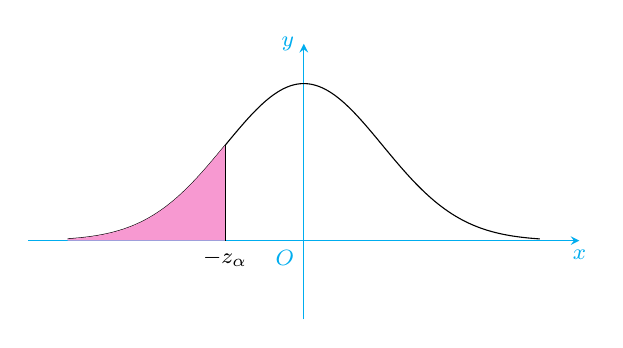
\begin{tikzpicture}[->,samples=100,>=stealth,font=\footnotesize,yscale=5]
            \def\xmin{-3.5}
            \def\xmax{3.5}
            \def\ymin{-.2}
            \def\ymax{.5}
            \def\a{0.398942}
            \draw[->,cyan](\xmin,0)--(0,0)node[below left]{$O$}--(\xmax,0)node[below]{$x$};
            \draw[->,cyan](0,\ymin)--(0,\ymax)node[left]{$y$};

            \draw[scale=1,domain=-3:3,smooth,variable=\x,black,-] plot ({\x},{\a*exp(-\x*\x/2)});

            % \fill[color=magenta!40] (1,0) -- plot[domain=1:3,smooth,variable=\x] ({\x},{\a*exp(-\x*\x/2)}) -- (3,0) --cycle;
            % \node[below] at (1,0) {$z_{\alpha/2}$};
            % \draw[-] (1,0)--plot[domain=1:1,smooth,variable=\x] ({\x},{\a*exp(-\x*\x/2)});

            \fill[color=magenta!40] (-1,0) -- plot[domain=-1:-3,smooth,variable=\x] ({\x},{\a*exp(-\x*\x/2)}) -- (-3,0) --cycle;
            \node[below] at (-1,0) {$-z_{\alpha}$};
            \draw[-] (-1,0)--plot[domain=-1:-1,smooth,variable=\x] ({\x},{\a*exp(-\x*\x/2)});
        \end{tikzpicture}
    }
    \caption{}
    \label{biaozfweidian}
\end{figure}

\begin{example}
    设总体 $X$ 服从正态分布 $N\qty(\mu,\sigma^2)$, $X_1, X_2, \cdots ,X_n$ 是来自总体 $X$ 的简单随机样本, 据此样本检验假设: $H_0:\mu=\mu_0,H_1:\mu\neq \mu_0$, 则
    \begin{tasks}
        \task 如果在检验水平 $\alpha=0.05$ 下拒绝 $H_0$, 那么在检验水平 $\alpha=0.01$ 下必拒绝 $H_0$.
        \task 如果在检验水平 $\alpha=0.05$ 下拒绝 $H_0$, 那么在检验水平 $\alpha=0.01$ 下必接受 $H_0$.
        \task 如果在检验水平 $\alpha=0.05$ 下接受 $H_0$, 那么在检验水平 $\alpha=0.01$ 下必拒绝 $H_0$.
        \task 如果在检验水平 $\alpha=0.05$ 下接受 $H_0$, 那么在检验水平 $\alpha=0.01$ 下必接受 $H_0$.
    \end{tasks}
\end{example}
\begin{solution}
    首先, 这是双边检验, 正态分布需要标准化, 作出标准正态分布的草图, $\alpha$ 是显著水平, 也是犯第一类错误的概率, 所以两边的阴影区域面积均为犯错概率,
    当 $\alpha$ 越小, 说明阴影区域面积越小, 中间非阴影区域部分为接受域, 这一部分会变大, 所以如果能在 $\alpha=0.05$ 时接受 $H_0$, 则必可以在 $\alpha=0.01$ 时接受 $H_0$, 故选 D.
\end{solution}

\begin{example}
    设某电子产品平均寿命 $ 5000 \mathrm{~h} $ 为达到标准, 现从一大批产品中抽出 $5$ 件, 试验结果 (单位: h) 如下:
    $$\begin{array}{lllll}
            5325 & 4878 & 4638 & 5652 & 4474
        \end{array}$$
    假设该产品的寿命 $ X \sim N(\mu, 1000)$, 试问此批产品是否合格 (取显著性水平 $ \alpha=0.05$)?
\end{example}
\begin{solution}
    由题意知, 需要检验假设
    $$H_0:\mu\geqslant 5000,~H_1:\mu<5000$$
    根据已知样本数据, 得 $ n=5, \bar{x}=4993, \sigma_{0}=\sqrt{1000} $, 则
    $$z=\frac{\bar{x}-\mu_{0}}{\sigma_{0} / \sqrt{n}}=\frac{\sqrt{5}(4993-5000)}{\sqrt{1000}}=-0.495$$
    查表知 $ z_{0.05}=1.645 $, 由于拒绝域为 $ z \leqslant-z_{\alpha}$, 故可接受 $ H_{0}$, 即认为该批产品合格.
\end{solution}

\subsubsection{\texorpdfstring{$\sigma^2$}. 未知, 关于 \texorpdfstring{$\mu$}. 的检验 (\texorpdfstring{$t$}. 检验)}

设总体 $ X \sim N\left(\mu, \sigma^{2}\right) $, 其中 $ \mu, \sigma^{2} $ 未知, 检验假设:
\begin{enumerate}[label=(\arabic{*})]
    \item 双边检验. $ H_{0}: \mu=\mu_{0} $, 备择假设 $ H_{1}: \mu \neq \mu_{0} $;
    \item 右边检验. $ H_{0}: \mu \leqslant \mu_{0}, H_{1}: \mu>\mu_{0}$ ;
    \item 左边检验. $ H_{0}: \mu \geqslant \mu_{0}, H_{1}: \mu<\mu_{0} $;
\end{enumerate}
这里以双边检验 $ H_{0}: \mu=\mu_{0}, H_{1}: \mu \neq \mu_{0} $ 为例求拒绝域.

若总体方差 $ \sigma^{2} $ 未知, $Z $ 检验法不能使用, 因为 $\displaystyle Z=\frac{\bar{X}-\mu_{0}}{\sigma / \sqrt{n}} $ 中含未知参数 $\sigma$, 不是统计量, 所以要选择其他的统计量来进行检验.
选取统计量 $\displaystyle t=\frac{\bar{X}-\mu_{0}}{S / \sqrt{n}} $ 作为检验统计量.
由抽样分布定理知, $\displaystyle\frac{\bar{X}-\mu_{0}}{S / \sqrt{n}} \sim t(n-1)$, 当原假设 $ H_{0} $ 成立时, 有
$$P_{\mu_{0}}\left\{\left|\frac{\bar{X}-\mu_{0}}{S / \sqrt{n}}\right| \geqslant t_{a / 2}(n-1)\right\}=\alpha$$
即得拒绝域为 $\displaystyle |t|=\left|\frac{\bar{x}-\mu_{0}}{s / \sqrt{n}}\right| \geqslant t_{\alpha / 2}(n-1)$.
类似地, 可得单边检验的拒绝域:
\begin{enumerate}[label=(\arabic{*})]
    \item 假设 $ H_{0}: \mu \leqslant \mu_{0}, H_{1}: \mu>\mu_{0}$, 其检验的拒绝域为 $ t \geqslant t_{\alpha}(n-1) $;
    \item 假设 $ H_{0}: \mu \geqslant \mu_{0}, H_{1}: \mu<\mu_{0}$, 其检验的拒绝域为 $ t \leqslant-t_{\alpha}(n-1) $.
\end{enumerate}
这种利用 $ t $ 统计量得出的检验法称为 $ t $ 检验法.

\begin{example}
    已知钢筋强度服从正态分布, 现测得生产出的钢筋强度 (单位: $ \mathrm{Pa} $) 分别为
    $$\begin{array}{lllll}
            55.5 & 59.0 & 53.5 & 51.5 & 56.0
        \end{array}$$
    能否认为其强度的均值为 $ 52.0(\alpha=0.05) $?
\end{example}
\begin{solution}
    在 $ \sigma^{2} $ 未知的条件下, 检验假设
    $$H_{0}: \mu=52.0, \quad H_{1}: \mu \neq 52.0$$
    选择统计量 $\displaystyle t=\frac{\bar{X}-\mu_{0}}{S / \sqrt{n}}$,
    由 $ n=5, \bar{x}=55.1, s=2.8151 $, 得统计量 $ t $ 的观测值为
    $$t=\frac{\bar{x}-\mu_{0}}{s / \sqrt{n}}=\frac{\sqrt{5}(55.1-52.0)}{2.8151}=2.4624$$
    当 $ \alpha=0.05 $, 查 $ t $ 分布表得临界值 $ t_{0.025}(4)=2.776 $, 由于 $ |t|=2.4624<2.776=t_{0.025}  (4)$, 所以接受假设 $ H_{0} $, 即认为钢笳强度的均值为 $ 52.0 $.
\end{solution}

\begin{example}
    已知某种电器在正常工作条件下平均消耗电流不会超过 $ 0.8 \mathrm{~A} $.
    现随机抽取 $16$ 台这种电器进行试验, 求得平均消耗电流为 $ 0.91 \mathrm{~A} $, 消耗电流的标准差为 $ 0.2 \mathrm{~A}$.
    假设电器所消耗的电流服从正态分布, 显著性水平为 $ \alpha=0.05$, 问能否认为电器在正常工作条件下平均消耗电流不会超过 $ 0.8 \mathrm{~A}$?
\end{example}
\begin{solution}
    根据题意, 检验假设
    $$H_{0}: \mu \leqslant 0.8, \quad H_{1}: \mu>0.8$$
    由于 $ \sigma $ 未知, 故采用 $ t $ 检验法, 选择检验统计量 $\displaystyle t=\frac{\bar{X}-\mu}{S / \sqrt{16}} \sim t(15) $,
    查表得 $ t_{0.05}(15)=  1.753$, 故拒绝域为 $\displaystyle \frac{\bar{x}-0.8}{s / \sqrt{n}}>1.753 $, 代人样本数据, 得 $\displaystyle t=\frac{\bar{x}-0.8}{s / \sqrt{n}}=\frac{0.9-0.8}{0.2 / \sqrt{16}}=2 $, 因此拒绝原假设, 即认为电器在正常工作条件下平均消耗电流会超过  $0.8 \mathrm{~A}$ .
\end{solution}

\begin{example}[1995 数三]
    设 $X_1, X_2, \cdots , X_n$ 是来自正态总体 $N\qty(\mu,\sigma^2)$ 的简单随机样本, 其中参数 $\mu$ 和 $\sigma^2$ 均未知, 记 $\bar{X}=\displaystyle \dfrac{1}{n}\sum_{i=1}^{n} X_i, Q^2=\sum_{i=1}^{n} \qty(X_i-\bar{X})^2$, 求假设 $H_0:\mu=0$ 的 $t$ 检验使用统计量.
\end{example}
\begin{solution}
    因为 $\sigma^2$ 未知, 故取统计量 $t=\dfrac{\bar{X}-\mu}{S/\sqrt{n}}$, 由 $\mu=0, S^2=\dfrac{Q^2}{n-1}$, 解得 $t=\dfrac{\bar{X}}{Q}\sqrt{n(n-1)}.$
\end{solution}

\subsubsection{\texorpdfstring{$\mu$}. 未知, 关于 \texorpdfstring{$\sigma^2$}. 的检验 (\texorpdfstring{$\chi^2$}. 检验)}

设总体 $ X \sim N\left(\mu, \sigma^{2}\right), \mu, \sigma^{2} $ 均未知, $X_{1}, X_{2}, \cdots, X_{n} $ 是来自 $ X $ 的样本, 要求检验假设 $ H_{0}: \sigma^{2}=\sigma_{0}^{2} ; H_{1}: \sigma^{2} \neq \sigma_{0}^{2}, \sigma_{0}^{2} $ 为已知常数 (显著性水平为 $ \alpha $).

选取 $\displaystyle \chi^{2}=\frac{(n-1) S^{2}}{\sigma_{0}^{2}} $ 作为检验统计量, 原假设 $ H_{0} $ 成立时, $\displaystyle \frac{(n-1) S^{2}}{\sigma_{0}^{2}} \sim \chi^{2}(n-1)$, 其拒绝域的形式为 $\displaystyle \frac{(n-1) s^{2}}{\sigma_{0}^{2}} \leqslant k_{1} $ 或 $\displaystyle \frac{(n-1) s^{2}}{\sigma_{0}^{2}} \geqslant k_{2} $, 其中 $ k_{1}, k_{2} $ 由下式确定:
$$\text{由 }  P\left\{ \right. \text{拒绝 }  H_{0} \mid H_{0} \left.  \text{ 为真}  \right\}=P_{\delta_{0}}\left\{\left(\frac{(n-1) S^{2}}{\sigma_{0}^{2}} \leqslant k_{1}\right) \cup\left(\frac{(n-1) S^{2}}{\sigma_{0}^{2}} \geqslant k_{2}\right)\right\}=\alpha$$
为计算方便, 习惯上取 $\displaystyle P_{\delta_{0}}\left\{\frac{(n-1) S^{2}}{\sigma_{0}^{2}} \leqslant k_{1}\right\}=\frac{\alpha}{2},~ P_{\delta_0}\left\{\frac{(n-1) S^{2}}{\sigma_{0}^{2}} \geqslant k_{2}\right\}=\frac{\alpha}{2} $, 得 $$ k_{1}=\chi_{1-\alpha / 2}^{2}(n-1) ,~  k_{2}=\chi_{\alpha / 2}^{2}(n-1) $$
于是拒绝域为
$$\frac{(n-1) s^{2}}{\sigma_{0}^{2}} \leqslant \chi_{1-\alpha / 2}^{2}(n-1) \quad \text { 或 } \quad \frac{(n-1) s^{2}}{\sigma_{0}^{2}} \geqslant \chi_{\alpha / 2}^{2}(n-1) .$$

类似地可得关于方差的两个单边检验的拒绝域:

\begin{enumerate}[label=(\arabic{*})]
    \item 假设 $ H_{0}: \sigma^{2} \leqslant \sigma_{0}^{2} ; H_{1}: \sigma^{2}>\sigma_{0}^{2} $, 该检验的拒绝域为 $\displaystyle \frac{(n-1) s^{2}}{\sigma_{0}^{2}} \geqslant \chi_{\alpha}^{2}(n-1) $;
    \item 假设 $ H_{0}: \sigma^{2} \geqslant \sigma_{0}^{2} ; H_{1}: \sigma^{2}<\sigma_{0}^{2} $, 该检验的拒绝域为 $\displaystyle \frac{(n-1) s^{2}}{\sigma_{0}^{2}} \leqslant \chi_{1-\alpha}^{2}(n-1) $.
\end{enumerate}
以上检验法称为 $ \chi^{2} $ 检验法.

\begin{example}
    某厂应用新工艺对加工好的 $15 $ 个活塞的直径进行测量, 得样本方差 $ s^{2}=  0.0006$.
    已知老工艺生产的活塞直径的方差为 $0.0004$. 问改革后活塞直径的方差是否不大于改革前的方差 (取显著性水平 $ \alpha=0.05$)?
\end{example}
\begin{solution}
    对方差进行右边检验, 且正态总体均值未知, 用 $ \chi^{2} $ 检验法.
    设测量值 $ X \sim N\left(\mu, \sigma^{2}\right), \sigma^{2}=0.0004 $.
    检验假设为
    $$H_{0}: \sigma^{2} \leqslant 0.0004, \quad H_{1}: \sigma^{2}>0.0004 $$
    选择统计量 $\displaystyle \chi^{2}=\frac{(n-1) S^{2}}{\sigma_{0}^{2}} $, 拒绝域为 $ \chi^{2} \geqslant \chi_{\alpha}^{2}(n-1) $.
    查表得 $ \chi_{0.05}^{2}(14)=23.685$, 代人样本数据, 得 $$\displaystyle \chi^{2}=\frac{(15-1) \times 0.0006}{0.0004}=21<23.685 $$
    故接受 $ H_{0} $, 即改革后活塞直径的方差不显著大于改革前的方差.
\end{solution}

\begin{example}
    若总体 $X\sim N\qty(0,\sigma^2)$, 对于总体 $X$ 的一个容量为 $n$ 的简单随机样本 $X_1, X_2, \cdots ,X_n$, 欲检验 $H_0:\sigma^2=4,H_1:\sigma^2\neq 4$, 则应选统计量
    \begin{tasks}(4)
        \task $\dfrac{(n-1)S^2}{4}$.
        \task $\dfrac{\sqrt{n}}{2}\bar{X}$.
        \task $\dfrac{1}{4}\displaystyle \sum_{i=1}^{n} X_i^2$.
        \task $\dfrac{\sqrt{n}}{S}\bar{X}$.
    \end{tasks}
\end{example}
\begin{solution}
    $X\sim N\qty(0,\sigma^2)$, 检验 $H_0:\sigma^2=4,H_1:\sigma^2\neq 4$, 由于 $\mu$ 已知, 应选统计量
    $$
        \chi^2=\dfrac{\displaystyle \sum_{i=1}^{n} \qty(X_i-\mu)^2}{\sigma_0^2}
    $$
    因为 $\sigma_0^2=4, \mu=0$, 即 $\chi^2=\displaystyle \dfrac{1}{4}\sum_{i=1}^{n} X_i^2$, 选 C.
\end{solution}

\subsection{双正态总体的假设检验}

%TODO

\subsubsection{双正态总体均值的检验 (\texorpdfstring{$t$}. 检验)}

\subsubsection{双正态总体方差的假设检验}

正态总体方差的假设检验各情况表.
\setcounter{magicrownumbers}{0}
\begin{table}[H]
    \centering
    \caption{正态总体方差的假设检验}
    \resizebox{.99\textwidth}{!}{
        \begin{tabular}{ccccl}
            \textbf{条件}                                 & \textbf{原假设}                      & \textbf{统计量}                                                                                                   & \textbf{对应样本函数分布}                                                        & \textbf{拒绝域}                                       \\
            \toprule
            \multicolumn{5}{c}{单正态总体均值和方差的假}                                                                                                                                                                                                                                                                                                        \\
            \midrule
            \multirow{3}{*}{已知 $\sigma^2$}              & $H_0:\mu=\mu_0$                      & \multirow{3}{*}{$Z=\dfrac{\bar{X}-\mu_0}{\sigma/\sqrt{n}}$}                                                       & \multirow{3}{*}{$N(0,1)$}                                                        & $|z|\geqslant z_{\alpha/2}$                           \\
                                                          & $H_0:\mu\leqslant \mu_0$             &                                                                                                                   &                                                                                  & $z\geqslant z_\alpha$                                 \\
                                                          & $H_0:\mu\geqslant \mu_0$             &                                                                                                                   &                                                                                  & $z\leqslant -z_\alpha $                               \\
            \midrule
            \multirow{3}{*}{未知 $\sigma^2$}              & $H_0:\mu=\mu_0$                      & \multirow{3}{*}{$t=\dfrac{\bar{X}-\mu_0}{S/\sqrt{n}}$}                                                            & \multirow{3}{*}{$t(n-1)$}                                                        & $|t|\geqslant t_{\alpha/2}(n_1+n_2-2)$                \\
                                                          & $H_0:\mu\leqslant \mu_0$             &                                                                                                                   &                                                                                  & $t\geqslant t_{\alpha}(n_1+n_2-2)$                    \\
                                                          & $H_0:\mu\geqslant \mu_0$             &                                                                                                                   &                                                                                  & $t\leqslant -t_{\alpha}(n_1+n_2-2)$                   \\
            \midrule
            \multirow{3}{*}{未知 $\mu$}                   & $H_0:\sigma^2=\sigma_0^2$            & \multirow{3}{*}{$\chi^2=\dfrac{(n-1)S^2}{\sigma_0^2}$}                                                            & \multirow{3}{*}{$\chi^2(n-1)$}                                                   & \makecell[l]{$\chi^2\geqslant \chi^2_{\alpha/2}(n-1)$ \\ $\chi^2\leqslant \chi_{1-\frac{\alpha}{2}}^2(n-1)$} \\
                                                          & $H_0:\sigma^2\leqslant \sigma_0^2$   &                                                                                                                   &                                                                                  & $\chi^2\geqslant \chi^2_\alpha(n-1)$                  \\
                                                          & $H_0:\sigma^2\geqslant \sigma_0^2$   &                                                                                                                   &                                                                                  & $\chi^2\leqslant \chi^2_{1-\alpha}(n-1)$              \\
            \midrule
            \multirow{3}{*}{已知 $\mu$}                   & $H_0:\mu=\mu_0$                      &                                                                                                                   &                                                                                  & \makecell[l]{$\chi^2\geqslant \chi^2_{\alpha/2}(n)$   \\ $\chi^2\leqslant \chi_{1-\frac{\alpha}{2}}^2(n)$} \\
                                                          & $H_0:\sigma^2\leqslant \sigma_0^2$   & $\chi^2=\dfrac{\displaystyle \sum_{i=1}^{n} (X_i-\mu)^2}{\sigma_0^2}$                                             & $\chi^2(n)$                                                                      & $\chi^2\geqslant \chi^2_\alpha(n)$                    \\
                                                          & $H_0:\sigma^2\geqslant \sigma_0^2$   &                                                                                                                   &                                                                                  & $\chi^2\leqslant \chi^2_{1-\alpha}(n)$                \\
            \midrule
            \multicolumn{5}{c}{双正态总体均值和方差的假}                                                                                                                                                                                                                                                                                                        \\
            \midrule
            \multirow{3}{*}{已知 $\sigma_1^2,\sigma_2^2$} & $H_0:\mu_1-\mu_2=\delta$             & \multirow{3}{*}{$Z=\dfrac{\qty(\bar{X}-\bar{Y})-\sigma}{\sqrt{\dfrac{\sigma_1^2}{n_1}+\dfrac{\sigma_2^2}{n_2}}}$} & \multirow{3}{*}{$N(0,1)$}                                                        & $|z|\geqslant z_{\alpha/2}$                           \\
                                                          & $H_0:\mu_1-\mu_2\leqslant \delta$    &                                                                                                                   &                                                                                  & $z\geqslant z_\alpha$                                 \\
                                                          & $H_0:\mu_1-\mu_2\geqslant \delta$    &                                                                                                                   &                                                                                  & $z\leqslant -z_\alpha $                               \\
            \midrule
            \multirow{3}{*}{未知 $\sigma_1^2=\sigma_2^2$} & $H_0:\mu_1-\mu_2=\delta$             & \multirow{3}{*}{$t=\dfrac{\qty(\bar{X}-\bar{Y})-\delta}{S_w\sqrt{\dfrac{1}{n_1}+\dfrac{1}{n_2}}}$}                & \multirow{3}{*}{$t(n_1+n_2-2)$}                                                  & $|t|\geqslant t_{\alpha/2}(n_1+n_2-2)$                \\
                                                          & $H_0:\mu_1-\mu_2\leqslant \delta$    &                                                                                                                   &                                                                                  & $t\geqslant t_{\alpha}(n_1+n_2-2)$                    \\
                                                          & $H_0:\mu_1-\mu_2\geqslant \delta$    &                                                                                                                   &                                                                                  & $t\leqslant -t_{\alpha}(n_1+n_2-2)$                   \\
            \midrule
            \multirow{3}{*}{未知 $\mu_1,\mu_2$}           & $H_0:\sigma_1^2=\sigma_2^2$          & \multirow{3}{*}{$F=\dfrac{S_1^2}{S_2^2}$}                                                                         & \multirow{3}{*}{$\dfrac{S_1^2/S_2^2}{\sigma_1^2/\sigma_2^2}\sim F(n_1-1,n_2-1)$} & $F\geqslant F_{\alpha/2}(n_1-1,n_2-1)$                \\
                                                          & $H_0:\sigma_1^2\leqslant \sigma_2^2$ &                                                                                                                   &                                                                                  & $F\geqslant F_\alpha(n_1-1,n_2-1)$                    \\
                                                          & $H_0:\sigma_1^2\geqslant \sigma_2^2$ &                                                                                                                   &                                                                                  & $F\leqslant F_{1-\alpha}(n_1-1,n_2-1)$
        \end{tabular}}
\end{table}

